\appendix


\section{Superlinear theorems}

\begin{theorem}
	\label{thm:superlinear}
	Superlinear
\end{theorem}

\begin{observation}
	\label{obs:list}
\end{observation}


\subsection{An upper bound on scaling of self-adjusting systems}

\maciek{Finished here}

The main finding of this section is that the superlinearity cannot continue forever.


Theorem. r is a function of , and on $k$ and $s$.


We aim to show a scaling law 



In the run of the system for the input $\sigma$, the serial part is to compute the load balancer's assignment, $s$, and the parallel part is to process the requests by the self-adjusting data structures, $1-s$.






Self-adjusting data structures scaled horizontally with load 



We observe two 



Superlinear speedup is a product of two simultaneous speedup factors: one $r\times$ speedup comes from the self-adjusting list getting progressively faster as the load balancer partitions the input better, and another $k\times$ speedup because we extend the total compute capacity available to the system $k$ times. The effective speedup is then just the multiple of the two, yielding $k^2$ times speedup in total. Plugging into Amdahl's law we get the \emph{scaling law for distributed MTF lists on uniform input} (see Fig.~\ref{fig:amdahl}):
\begin{equation}\label{eq:mtf-perf}
  S_l(k) = \frac{T_l(1)}{T_l(k)} = \frac1{s + \frac{1-s}{k^2}} \enspace .
\end{equation}






- consider a horizontally scaled architecture of self-adjusting data structures managed by any load balancer

- Our baseline is an algorithm that uses a load-balancer (incurs the same cost per item -- can vary with items, but is uniquely determined by the item, lbtime(it)), and is a single self-adjusting data structure.

- However, the main point of this comparison: in the self-adjusting world, the simplest baseline is the non-scaled reference point. It is the simplest to reason about, and the self-adjusting Amdahl's law gives initial superlinear scaling in such an approach.


\subsection{Relations to Amdahl's law}

The baseline choice is crucial for the benchmark to show superlinear scaling.
In reality, even locally we should use the best possible algorithm, a sophisticated load-balancers to break-down self-adjusting data structures.
With such a perspective, the baseline changes, and Amdahl's law applies.

\subsection{Our Results Overview}

First, we show an upper bound in this supposedly uneven benchmark.
It shows that the superlinear scaling cannot continue with k indefinitely. Rather, it hits a limit for some value of k.

Even if superlinear scaling is an ephemeral phenomena, under good conditions we may enjoy it in \emph{inital} growth with k.
The good conditions are: the system's cost model follows the working set property. The load balancer breaks working sets (increases locality).

% In our architecture, scaling is not dependent on the number of machines, but rather on the effectiveness of the load balancer to break working sets.
% Our architecture fixes the number of load-balancer "server affinity" domain linearly growing with the number of machines.







A system \emph{scales superlinearly} if baseline/system follows Amdahl with k:=k times r for an infinite set of input sequences (carefully constructed below). There is s in this equation.




\subsection{Upper-bound on superlinear scaling of self-adjusting data structures.}

definitions.
Input sigma.
Self-adjusting data structure's cost.
LB savings.

We aim to give a common upper bound for parallel scaling of caching, self-adjusting lists and splay trees.

- all these can be captured by varying access cost



\begin{theorem}
 We upper-bound the total scaling (scaled / baseline) latency in finishing the jobs by k := k times r in Amdahl, where r is obtained by -(cost saved due to working set breaking)).

* objective: completion time
* for an upper bound, we can take a perspective of average load over time (?) to upper bound completion time, assuming best machine scheduling and load balancing
* so, how does the total work behave?
    * we have -r for the cost reduced from the baseline, which is a single self-adjusting data structure that needs to incur the cost of load-balancing too.

* then, scaling is a product of machine scaling and load-balancing savings -r

 
\end{theorem}

\begin{proof}
  by working sets breaking, total work argument, and Amdahl
\end{proof}

* link to theorems with more thorough characterization:
    * upper bound of opt for caching Albers
    * upper bound on opt for list access locality Albers
    * why these are useful?


An immediate corrolary is that caching superlinear scaling eventually ends for a fixed cache size per machine and a finite universe of items (do we need the 2nd assumption?)


\subsection{Initial superlinear scaling by locality-boosting load balancers.}



A locality boosting load balancer is defined then by any growth of r as a function of k. It may give initial superlinear scaling (performance gain in terms of k).

Corollary: We should adapt some algorithm-specific logic to the load-balancer to achieve superlinear scaling.



\subsection{1}


We can grab the fruits of localisty boosting lb even to break single core sa datastructures. However  this is best combined worth scaling of machines. We should maximize balancing on a single machine first. Then, adding manny machines reduces registers contention




Caching is also subject to initial only scaling. How to show? In appendix 4. By Albers, another paper gives a limit on opt in terms of f. Eventually, no more f to decrease by lb, and superlinearity ends. Does scaling work if we share a cache of some size l without scalong number of machines? It actually can hurt you (associate caching, only some items occupy certain space, it is weaker. How gains can be made? Say we split in two, and there are 2l items requested round robin. Then, lru page faults all time. But if we manage to cut out k/2 items that stay in cache, we only page fault 7t% of time.


A corollary is that we should not only design self adjusting data structures for where the input has locality. But we should design them in tandems, with locality boositing lbs, that need to be designed for a given data structure solution to a problem. Lbs should retain their usual properties such as sticyness and evening the load among machines.

More complicated situation. No multiplying in amdahl, but a subtraction. However, we can express it this way to have scaling factor like superlinear by multiplying it as a fraction of 1-s, to get the same classification. See concept notes for derivation of the formula with R standards scaling form. This works for cachong too


If the benchmark for scaling would be the lb single core with locakity broken, the superlinearity would not hold. However, it holds wrt. A single algorithm that is non-efficient is then used as a baseline.




Why is this phenomenon an argument for using self adjusting ds? When lb done right, we haveand effect of both k and r multiplied. In this architecture.

Outcomes of the paper. Scaling sa ds requires careful load balancing. We can ruin performance or boost it more than linearly.

Ripe the benefits of scaling with a simple architecture that is horizontally scalable.



On superlinear performance improvements of horizontally scaled self adjusting ds with good load balancing pattern.


\subsection{2}





As an interesting corollary, it should also imply that superlinear scaling for caching (with load balancing) is only an initial phenomenon.







Universal scaling law.

First, let r be the savings by cutting with lb on single core. This reduces total work by r (normalize so it is not N, but at most 1). Then, define R in terms of s and r. Then, amdahl says that the scaling is ..R*k.


Consider a load balancer and k parallel machines according to our horizontally scaling architecture. Fix input sigma and a self adjusting data structure. Let t(1) be the performance of a single ds on sigma.




Let s be the serial part (compute the load balancing primitive in this case).




Let l be the lb work, and s be the single data structure running time. Then, a single core has cost of s. And k machines have work of l+(s-r)/k= l+s/(k*R) by at most perfect split of s and by locality boosting bonus.

If the single core must calculate lb for some reason. Then l+s=1, and the law is as for amdahl.


\subsection{3}



* Mrf is only harder
* Caching is not s generalization of mtf, it's mtf in different cost model (sleator cite). Say that mtf is lru
* Load-balance yourself out to superlinear scaling
* Add my related work
* Discussion about retaining good properties of lbs, such as uniform balanicing
* Appendix. We simplify the spatial dimension to two items. Then runs perfectly capture temporal locality. And there is independence between pairs, amd the costs add up
* Evaluations. Sleep is maybe bad, because it allows for other threads? Instead, random numbers generation in batches.
* Say stateless classifier
* The rss link to cut based partitioning? In the intro, abstract, main
* Todo. Think how to explain single core scaling. This analysis is in case of mtf exact search and sticky hashing. But it is more general, and we can use efficuts like to have the same analysis for packet classification. There are overlaps in each partitioning, where we retain some runs (assigned to different cores) in the cost.
* Hash table degeneration not always possible. If only one core scaling, it is not superlinear, but we see scaling nonetheless. Superlinear comes from combining these scaling. We do it by changing the objective to total avg work /cores, assumming it is uniform (cheating, todo rss+). Say this is future work.
* B
* Is there a limit to superlinear scaling? Yes, this is initial scaling. In the extreme, no self adjustments help. Describe this limitation. On a good side, the initial scaling is practical
* B
* Formulas for the objective todo. That also take the parallel scaling into account. Say, we assume perfect load balancing with avg load minimization, which is already captured. But what is really going on is limiting the scaling. The correct objective is.
* The objective. Batches of packets arrive, and need to be processed. We progress to the next batch when all are finished. Then bad improvement, say we cannot batch. The objective is sum completion times.
* Say we do not batch, then we need to process in parallel many requests. If we can scale the single core load (beyond this paper, wait for rss or employ many cores in a single traversal of a long path).
* The superlinear scaling clearly vanishes when there are no more runs to cut. Its however not a quadratic number of runs to cut, since each cut partitions into two, cutting at least linear number of edges.
* To obtain perfect superlinear scaling, one must break all runs, maybe even dynamically changing the partition




Caches and lru are similar, but the function f is general. No longer we
* No longer we care about each overtake, but about the events that there are k overlaps. For lru. Since these are correlated with number of overtakse, we can conclude that it can be analyzed similarly, but we focus on lists.
* Caches cannot be scaled single core. I.e. they could be, but we need more memory, so its a bigger machine.

\subsection{4}



The section 3.3 splits superlinear into the product  of (1) extra  capacity and (2) self-adjustments. Gabor wrote there $k^2$ in modified amdahl. But the self-adjustment gains do not scale with k. Rather, the second factor(call it r) is a new parameter for locality boosting.This gives us a product of k and r (not $k^2$) in amdahl. The parameter  r is based on the input sequence (rules and packets) and datastructure, independently of k. Locality boosting is tied to the concept of "broken runs", explained in the appendix.

Then, we need to explain why our law has a product, not say, min or max of r and k. But k*r is indeed an upper bound for parallel lists that follow the standard list cost model  (proof by an argument of total work, and a rough upper bound of perfect work sharing).

Scaling cannot increase superlinearly forever because at some point there is no more runs to break. Hence superlinear scaling is only initial. As we scale the number k, in our system design, load balancing also affects r. But the effect of LB on r can be even much larger in k.

Locality boosting load balancing system is defined then by any growth of r as a function of k.



Our Amdahl law for self-adjusting systems is hence not a generalization of Amdahl, but its application to self adjusting systems (This is proven by performance improvements in single-core). We introduce another parameter related to self-adjusting  data structures (locality boosting parameter r).










Our scaling law however generalizes locality analysis for mtf (Albers) in distributed setting.

\subsection{5}



In the appendix we explain the paradox of the single cpu performance improvements with LB.

We state the performance of partitioned mtf lists in terms of input locality. This is the simplest cost model for LB+self-adjusting, without parallelism.

The theorem of Albers that we use is tight, in a sense that it is not an upper or a lower bound, it's exactly the cost, so our bounds are strong. Our characterization also generalizes to the mrf m.








In the appendix we analytically explain the paradox of the single cpu performance improvements with LB.

We state the performance of partitioned mtf lists in terms of input locality. This is the simplest cost model for LB+self-adjusting for lists.

The theorem of Albers that we use is tight, in a sense that it is not an upper or a lower bound, it's exactly the cost, so our bounds are strong. Our characterization also generalizes to the mrf model.

The model also explains parallelism gains, but only for the objective of total work minimization, not completion time.

\section{Locality-boosting analysis}

I'll take care of this section. Maciek.


Definitions are in Section~\ref{sec:locality-boosting}

Locality-boosting gains depend on the ability to choose a partitioning that isolates requests with similar access patterns.
Consider a self-adjusting list
storing a set of items $\{ 1, 2, 3, 4, 5, 6 \}$, and consider a request sequence $\sigma = \langle 1, 2, 3, 1, 2, 3, 1, 2, 3, \ldots \rangle$.
If the items are stored in a single self-adjusting list with a Move-To-Front reorganization operation, the three requested items $\{1,2,3\}$ compete for the front of the list, and incur the cost of three comparisons per each request.
However, if we partition the items into three lists with a partitioning function that assigns the items $\{1, 2, 3\}$ to different lists, then the requested items would occupy the front of their respective lists, resulting in one comparison per request.

\subsection{Analysis}
% \subsubsection{Absolute costs for a single self-adjusting list.}
% Self-adjusting lists are often analyzed within the framework \emph{competitive analysis}~\cite{Borodin98}, where we compare the online algorithm's performance to an offline optimum for the sequence.
% However, in this work we are interested in absolute costs.

Albers and Lauer~\cite{AlbersL16} characterized the absolute cost of serving a request sequence $\sigma$ in terms of the number of \emph{runs} in $\sigma$.
Runs are defined for two-item input sequences, and to characterize sequences consisting of more items, we sum the number of runs in sequences with all but two items removed, for all pairs of items.

\begin{definition}
	Let L be the set of items in the list to be maintained. Consider a fixed request sequence~$\sigma$. For any two items $x, y \in L$
	with $x \neq y$, let $\sigma_{xy}$ be the request sequence that is derived from $\sigma$ by deleting all requests that are neither to x nor
	to y.
\end{definition}

\begin{definition}
	Any maximal subsequence of consecutive requests to the same item in $\sigma_{xy}$ is called a run. Let $r(\sigma_{xy})$ be the number of runs in $\sigma_{xy}$. 
	We define $r(\sigma) = \sum_{x,y : x \neq y} r(\sigma_{xy})$.
\end{definition}
%
Then, the cost of Move-To-Front can be upper-bounded in terms of number of runs:
%
\begin{theorem}
	For any sequence $\sigma$ the cost incurred on a single list by MTF is 
	$MTF(\sigma) \le r(\sigma) + |\sigma|$.
	\label{thm:mtf-runs}
\end{theorem}
The proof of the above theorem is due to Albers and Lauer~\cite{AlbersL16}.

The above characterization in terms of runs can be extended to partitioned self-adjusting lists running Move-To-Front.
\begin{lemma}
	For each list $L_i$, let $\sigma^{(h(\cdot) = i)}$ be a subsequence of the input $\sigma$ that contains only requests to the items assigned by $h$ to $L_i$.
	The total absolute cost incurred is then:
	$$
	MTF_h(\sigma) \le (\sum_{1 \le i \le m} r(\sigma^{(h(\cdot) = i)})) + |\sigma|
	$$
	\label{lem:parallel-cost-mtf}
\end{lemma}
\begin{proof}
	The proof follows by summing up the cost of Move-To-Front in each individual list, followed by Theorem~\ref{thm:mtf-runs}:
	
	$$ MTF_h(\sigma) \le \sum_{1 \le i \le k} (r(\sigma^{(h(\cdot) = i)}) + |\sigma^{(h(\cdot) = i)}|) = (\sum_{1 \le i \le k} r(\sigma^{(h(\cdot) = i)})) + |\sigma|,$$
	where the last step follows as $h$ is a function, and it assigns each item to only one list.
\end{proof}
The above cost characterization depends then on $h$, the assignment of items to lists.

We compare the cost incurred by the parallel lists $MTF_h(\sigma)$ to the cost incurred on a single list, $MTF(\sigma)$, in terms of the function $h$.
To this end, we define a \emph{run graph} of a sequence $\sigma$.
\begin{definition}
	For a given sequence $\sigma$, a \emph{run graph} is a complete weighted graph on $n$ vertices, where the weight of an edge $(x,y)$ is $r(\sigma_{xy})$.
\end{definition}

For an example of a run graph with hash functions, see Figure~\ref{fig:example}.
In this example, we consider two partitioned lists containing four items $a,b,c$ and $d$, and an input sequence $\sigma := abababacacaccacacadc$, $|\sigma| = 20$.
Then, $\sigma_{ab} = abababaaaaaa$ consist of $7$ runs, $\sigma_{ac} = aaaacacaccacacac$ consists of 12 runs, 
$\sigma_{ad} = aaaaaaaaad$ consists of 2 runs, 
$\sigma_{bc} = bbbccccccc$ consists of 2 runs,  $\sigma_{bd} = bbbd$ consist of 2 runs and $\sigma_{cd} := ccccccdc$ consists of 3 runs.
Figure~\ref{fig:example} depicts the run graph for $\sigma$ and two examples of functions $h_1$ and $h_2$, with $w(C_{h_1}) = 18$ and $w(C_{h_2}) = 21$ being the savings from choosing an assignment $h_1$ or $h_2$, respectively.


\begin{figure}[h!]
	\center
	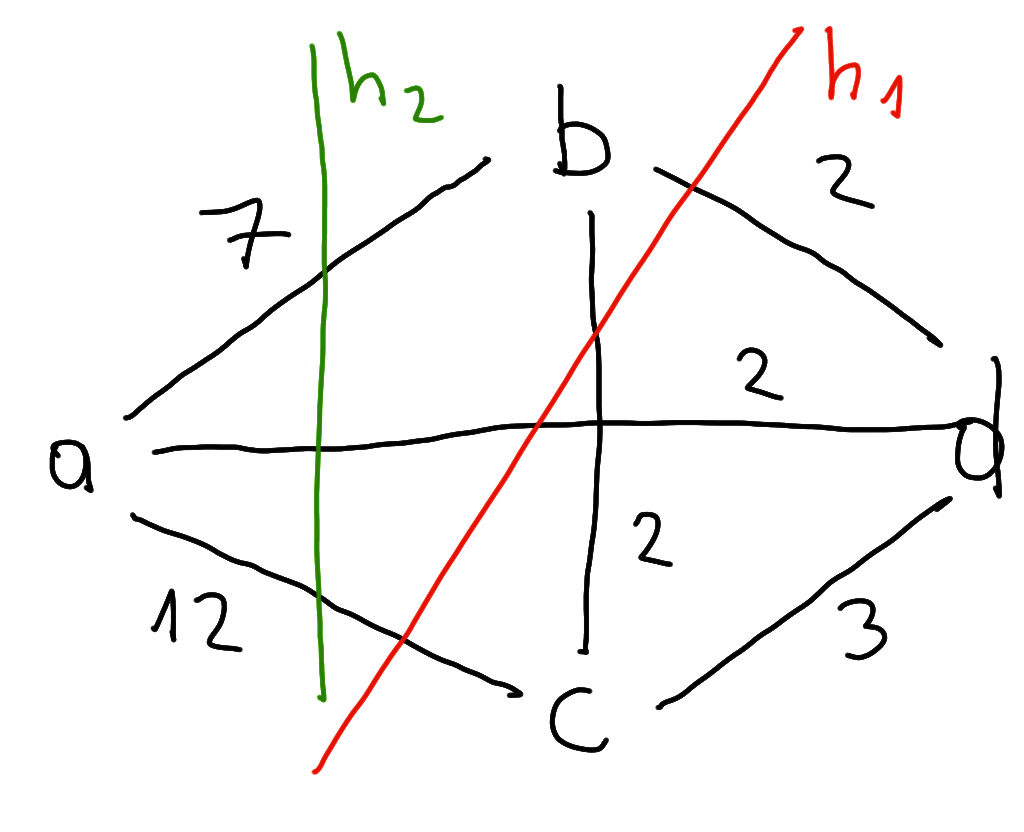
\includegraphics[width=0.5\textwidth]{./fig/cut.png}
	\caption{The run graph for $\sigma = abababacacaccacacadc$ and two examples of functions $h_1$ and $h_2$, with $w(C_{h_1}) = 18$ and $w(C_{h_2}) = 21$.}
	\label{fig:example}
\end{figure}




The run graph helps in characterizing the gains from the partitioning schema.
Each function $h$ induces a $k$-way cut of the run graph, denoted $C_h$.
With this characterization, we express the cost of parallel lists in comparison to the cost of a single list.
\begin{observation}
	Let $M$ be the cost incurred by $MTF$ operating on a single list.
	Then, the cost incurred by parallel $MTF_h$ is at most $M - w(C_h)$, where $w(C_h)$ is the total weight of the $k$-way cut $C_h$ induced by $h$.
\end{observation}

The observation follows by summing up the costs for individual lists with Lemma~\ref{lem:parallel-cost-mtf}.

Note that we ignore the cost of computing the hash function, and account only for item comparisons.


%%% Local Variables:
%%% mode: latex
%%% TeX-master: "distributed_mrf"
%%% End:
